
\documentclass{beamer}

\usepackage{hyperref}
\usetheme{Singapore}
\usecolortheme[RGB={0, 32, 91}]{structure}  % Rice blue
\setbeamertemplate{navigation symbols}{\insertframenumber}

\definecolor{riceblue}{rgb}{0.000, 0.125, 0.357}
\definecolor{ricegray}{rgb}{0.486, 0.494, 0.498}
\definecolor{ricerichblue}{rgb}{0.039, 0.314, 0.620}

\title{Baseball pitch trajectory density estimation \\ for predicting future pitcher outcomes}
\author{\color{ricerichblue} Scott Powers and Vicente Iglesias}
\date{Conference of Texas Statisticians 2024}

\begin{document}

  \begin{frame}
    \maketitle
    \vfill
    \hfill
    
\includegraphics[width = 4cm]{images/rice_logo.png}
  \end{frame}

  \begin{frame}{The Problem}
    MLB teams spend A LOT of money on pitchers ...\\
    ~\\
    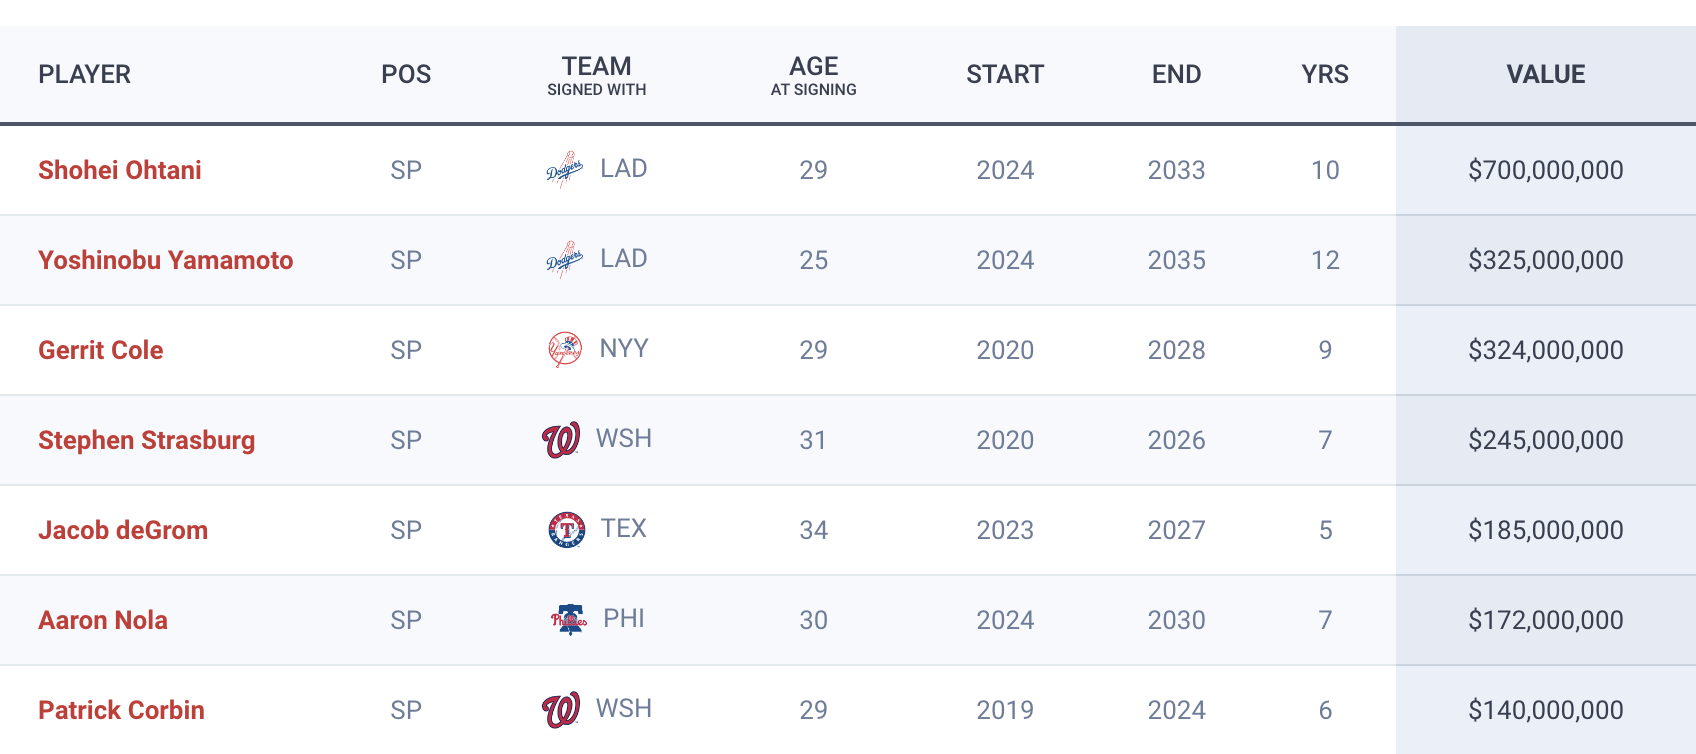
\includegraphics[width = \textwidth]{images/free_agent_contracts.png}\\
    \hfill{\scriptsize \color{ricegray} spotrac.com}\\
    ~\\
    \hfill ... and they don't always know who the best ones are.
  \end{frame}

  \begin{frame}{Standard of Practice}
    \begin{itemize}
      \item Observe $X \in \mathbb{R}^9$ describing each pitch trajectory
      \item Observe $Y \in \mathbb{R}$ describing the run value of the pitch outcome
      \item Estimate $f(x) = \mathbb{E}[Y \mid X = x]$
      \begin{itemize}
        \item This is a standard supervised learning problem
      \end{itemize}
      \item Evaluate the pitcher using $\frac1n\sum_{i = 1}^n \hat f(x_i)$
      \begin{itemize}
        \item This turns out to work better than using actual outcomes
      \end{itemize}
    \end{itemize}
    ~\\
    Let's call this the {\bf Descriptive} model, e.g. Healey (2019)
  \end{frame}

  \begin{frame}{The Conundrum}
    \begin{columns}
      \begin{column}{0.5\textwidth}
        \centering
        $\mbox{Variable Importance}^1$\\
        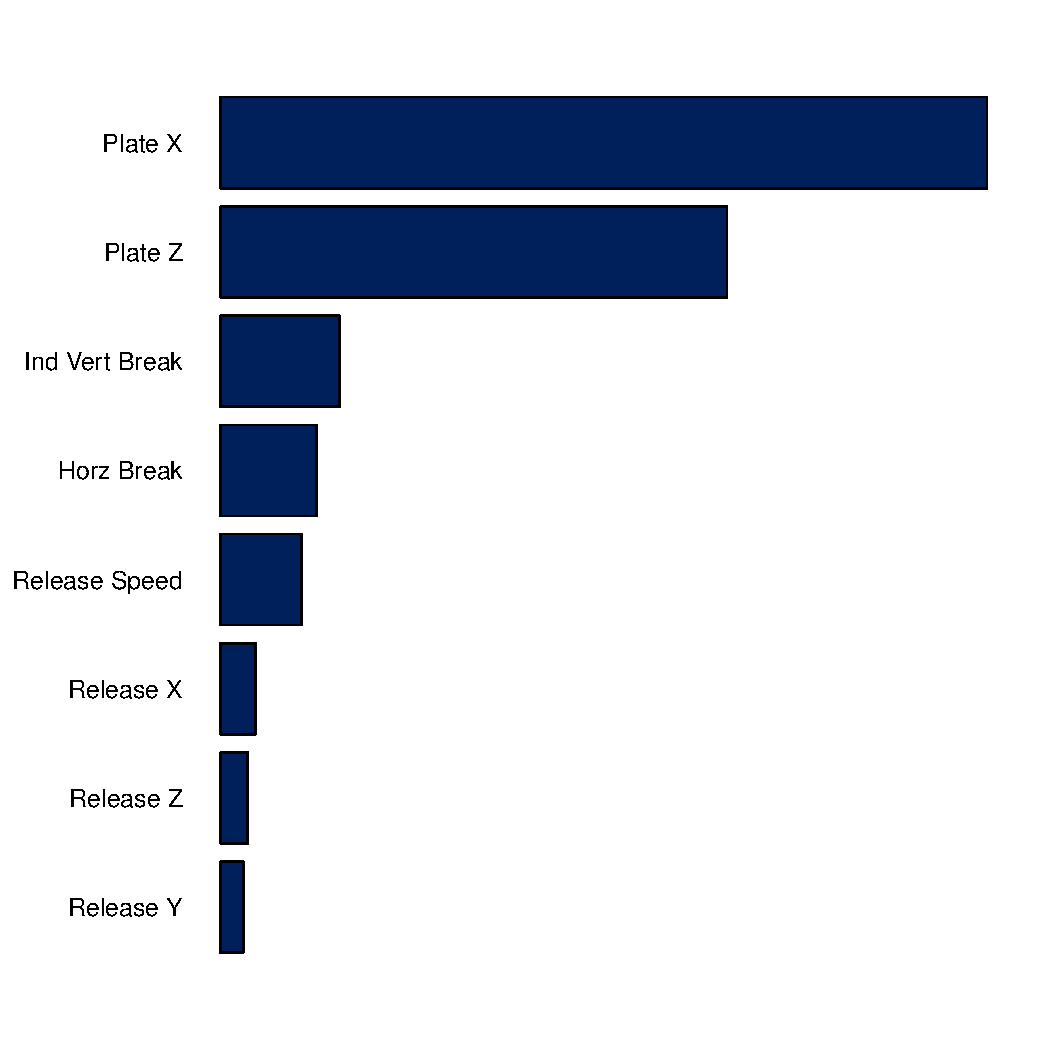
\includegraphics[width = \textwidth]{images/feature_importance.pdf}
      \end{column}
      \begin{column}{0.5\textwidth}
        \centering
        $\mbox{Variable Reliability}^2$\\
        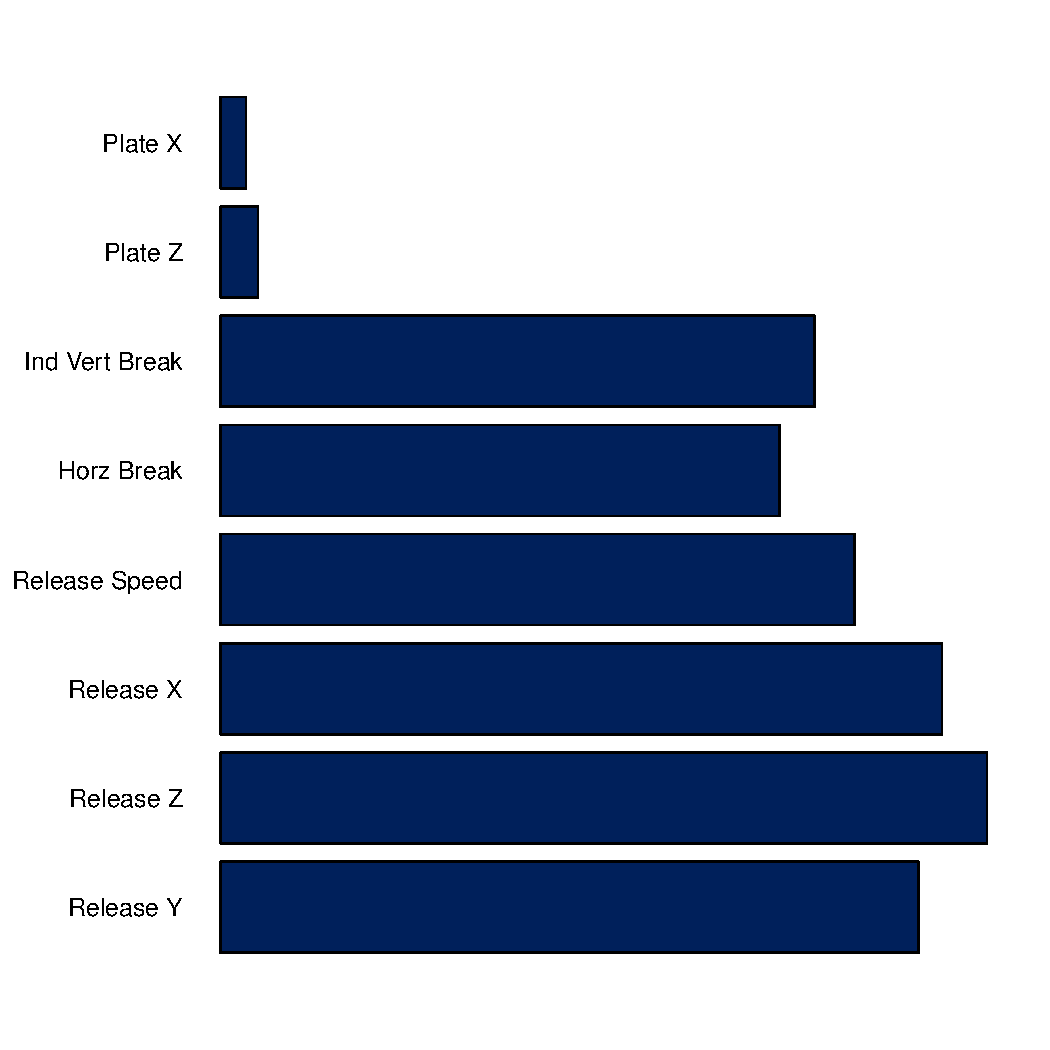
\includegraphics[width = \textwidth]{images/feature_reliability.pdf}
      \end{column}
    \end{columns}
    \scriptsize \color{ricegray}
    \vfill
    ${}^1$ fractional contribution of each feature's splits to gradient boosting pitch model\\
    ${}^2$ (between-pitcher variance) / (total variance); varies by pitch type (here: RHB FB)
  \end{frame}

  \begin{frame}{Why Supervised Learning Isn't Enough}
    \begin{columns}
      \begin{column}{0.4\columnwidth}
        \centering
        {\bf Supervised Learning}\\
        ~\\
        \begin{tabular}{ccc}
          Pitch &               & Outcome\\
          $x_1$ & $\rightarrow$ & $y_1$\\
          $x_2$ & $\rightarrow$ & $y_2$\\
          $x_3$ & $\rightarrow$ & $y_3$\\
                & ...           &      \\
          $x_n$ & $\rightarrow$ & $y_n$\\
          \\
          \\
          \\
          $x^*$ & $\rightarrow$ & $\hat y$\\
        \end{tabular}
      \end{column}
      \begin{column}{0.6\columnwidth}
        \centering
        {\bf Our Problem}\\
        ~\\
        \begin{tabular}{cccc}
          Pitcher & Pitch &               & Outcome\\
          A       & $x_1$ & $\rightarrow$ & $y_1$\\
          A       & $x_2$ & $\rightarrow$ & $y_2$\\
          B       & $x_3$ & $\rightarrow$ & $y_3$\\
                  &       & ...           &      \\
          C       & $x_n$ & $\rightarrow$ & $y_n$\\
                  & \\
                  &       & $\searrow$    & {\color{white} $\int\hat p(x)\hat f(x)$}\\
                  & \\
          A       &       &               & $\hat y$\\
        \end{tabular}
      \end{column}
    \end{columns}
  \end{frame}

  \begin{frame}{Why Supervised Learning Isn't Enough}
    \begin{columns}
      \begin{column}{0.4\columnwidth}
        \centering
        {\bf Supervised Learning}\\
        ~\\
        \begin{tabular}{ccc}
          Pitch &               & Outcome\\
          $x_1$ & $\rightarrow$ & $y_1$\\
          $x_2$ & $\rightarrow$ & $y_2$\\
          $x_3$ & $\rightarrow$ & $y_3$\\
                & ...           &      \\
          $x_n$ & $\rightarrow$ & $y_n$\\
          \\
          \\
          \\
          $x^*$ & $\rightarrow$ & $\hat y$\\
        \end{tabular}
      \end{column}
      \begin{column}{0.6\columnwidth}
        \centering
        {\bf \color{ricerichblue} Our Solution}\\
        ~\\
        \begin{tabular}{cccc}
          Pitcher & Pitch &               & Outcome\\
          A       & $x_1$ & $\rightarrow$ & $y_1$\\
          A       & $x_2$ & $\rightarrow$ & $y_2$\\
          B       & $x_3$ & $\rightarrow$ & $y_3$\\
                  &       & ...           &      \\
          C       & $x_n$ & $\rightarrow$ & $y_n$\\
                  & \\
                  & {\color{ricerichblue}$\downarrow$}\\
                  & \\
          A       & {\color{ricerichblue} $\hat p(x)$} & {\color{ricerichblue}$\rightarrow$} & {\color{ricerichblue} $\int\hat p(x)\hat f(x)$}\\
        \end{tabular}
      \end{column}
    \end{columns}
  \end{frame}

  \begin{frame}{Our Solution}
    \begin{enumerate}
      \item Estimate the probability distribution over pitch trajectories
      \begin{itemize}
        \item Depends on pitcher, batter side, count, etc.
        \item We use a Bayesian hierachical model to share information
        \item Expensive to sample from posterior (81 parameters per pitcher)
        \item We find MAP model fit using automatic differentiation
      \end{itemize}
      ~\\
      \item Fit a model to predict pitch outcome given its trajectory
      \begin{itemize}
        \item We use gradient boosting, not the focus today
      \end{itemize}
      ~\\
      \item Integrate the model {\color{riceblue} 2.} w.r.t. the distribution {\color{riceblue} 1.}
    \end{enumerate}
    ~\\
    Let's call this the {\bf Predictive} model
  \end{frame}

  \begin{frame}{Dylan Cease's Slider vs RHB in All Counts}
    \vfill
    \centering
    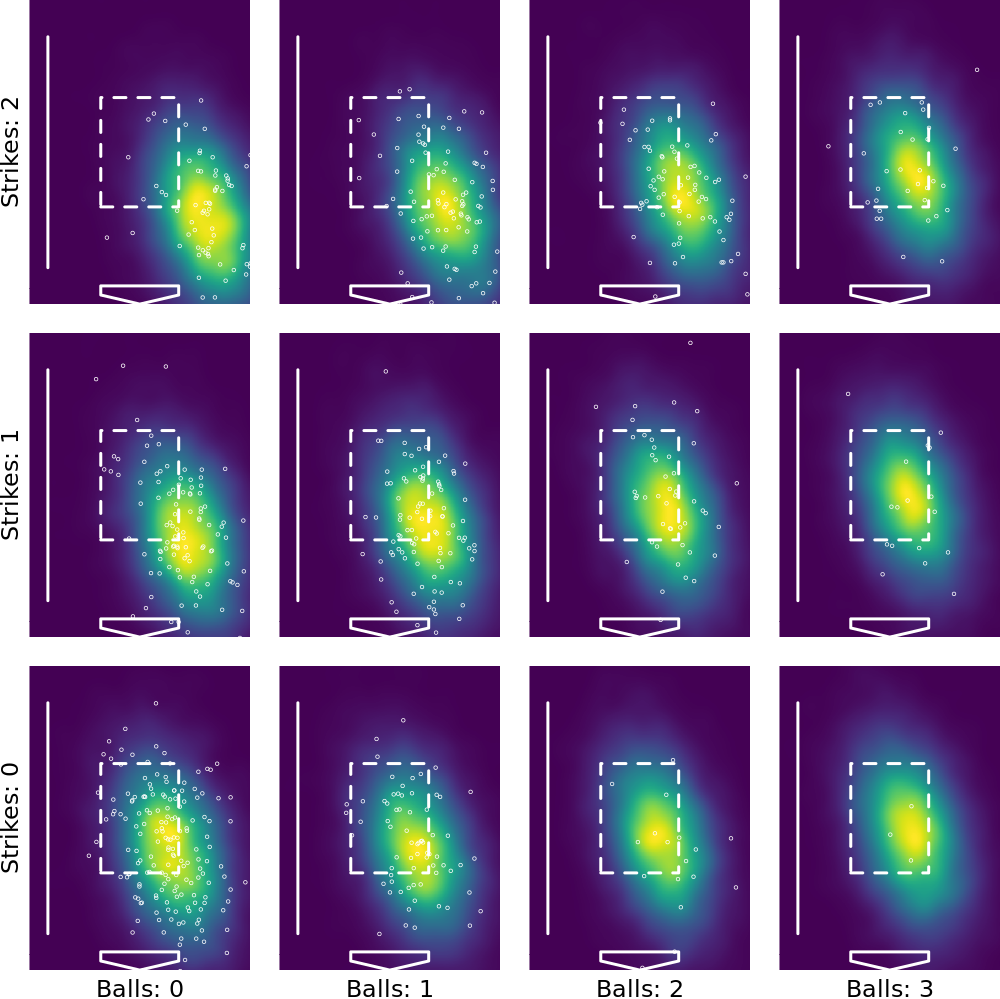
\includegraphics[height = 0.85\textheight]{images/656302_SL_R_plate.png}
  \end{frame}

  \begin{frame}{Does It Work?}
    \centering
    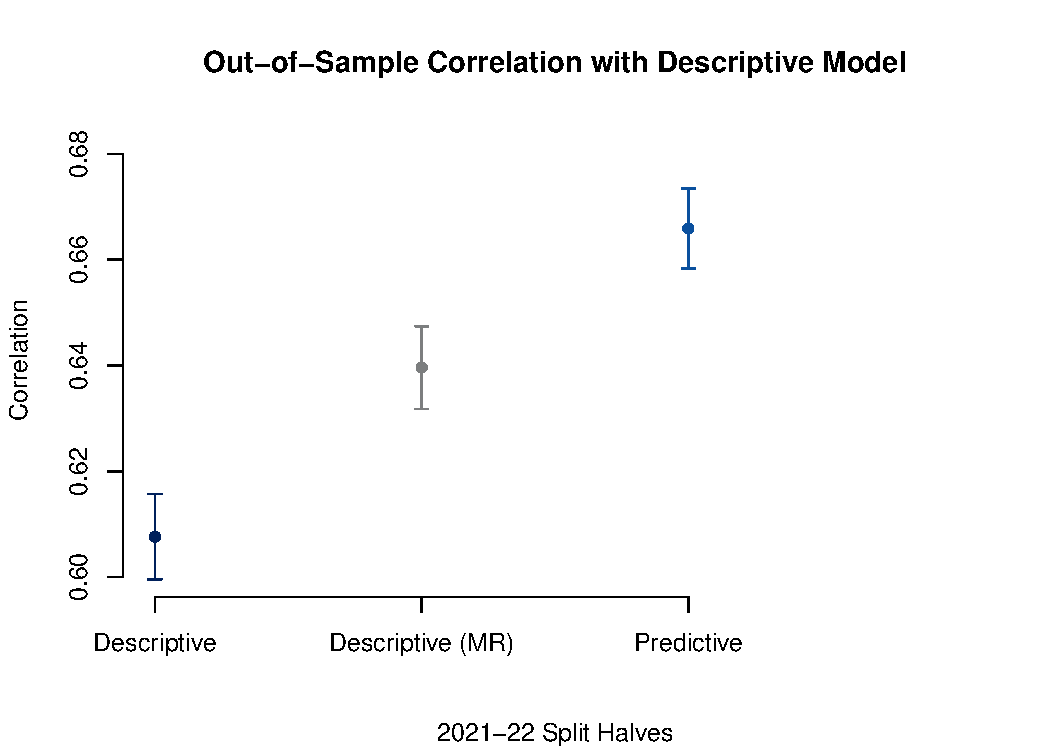
\includegraphics[width = \textwidth]{images/cor_overall_3.pdf}
  \end{frame}

  \begin{frame}{Next steps}
    \begin{itemize}
      \item Better (simpler?) parameterization for distribution model
      \item Relax Gaussian assumption (unimodal with specific tails)
    \end{itemize}
  \end{frame}

  \begin{frame}{Thank You!}
    \begin{center}
      \color{ricerichblue}saberpowers.github.io
    \end{center}
    \vfill
    \footnotesize
    References\\
    ~\\
    Healey G (2019) ``A Bayesian method for computing intrinsic pitch values using kernel density and nonparametric regression estimates'' {\it Journal of Quantitative Analysis in Sports} 15(1) 59-74
  \end{frame}

\end{document}
